\documentclass[paper=letter,11pt]{scrartcl}

\KOMAoptions{headinclude=true, footinclude=false}
\KOMAoptions{DIV=14, BCOR=5mm}
\KOMAoptions{numbers=noendperiod}
\KOMAoptions{parskip=half}
\addtokomafont{disposition}{\rmfamily}
\addtokomafont{part}{\LARGE}
\addtokomafont{descriptionlabel}{\rmfamily}
%\setkomafont{pageheadfoot}{\normalsize\sffamily}
\setkomafont{pagehead}{\normalsize\rmfamily}
%\setkomafont{publishers}{\normalsize\rmfamily}
\setkomafont{caption}{\normalfont\small}
\setcapindent{0pt}
\deffootnote[1em]{1em}{1em}{\textsuperscript{\thefootnotemark}\ }


\usepackage{amsmath}
\usepackage[varg]{txfonts}
\usepackage[T1]{fontenc}
\usepackage{graphicx}
\usepackage{xcolor}
\usepackage[american]{babel}
% hyperref is needed in many places, so include it here
\usepackage{hyperref}

\usepackage{xspace}
\usepackage{multirow}
\usepackage{float}


\usepackage{braket}
\usepackage{bbm}
\usepackage{relsize}
\usepackage{tcolorbox}

\def\ketY{\ensuremath{\ket {\Psi}}}
\def\iGeV{\ensuremath{\textrm{GeV}^{-1}}}
%\def\mp{\ensuremath{m_{\textrm{proton}}}}
\def\rp{\ensuremath{r_{\textrm{proton}}}}
\def\me{\ensuremath{m_{\textrm{electron}}}}
\def\aG{\ensuremath{\alpha_G}}
\def\rAtom{\ensuremath{r_{\textrm{atom}}}}
\def\rNucl{\ensuremath{r_{\textrm{nucleus}}}}
\def\GN{\ensuremath{\textrm{G}_\textrm{N}}}
\def\ketX{\ensuremath{\ket{\vec{x}}}}
\def\ve{\ensuremath{\vec{\epsilon}}}


\def\ABCDMatrix{\ensuremath{\begin{pmatrix} A &  B  \\ C  & D \end{pmatrix}}}
\def\xyprime{\ensuremath{\begin{pmatrix} x' \\ y' \end{pmatrix}}}
\def\xyprimeT{\ensuremath{\begin{pmatrix} x' &  y' \end{pmatrix}}}
\def\xy{\ensuremath{\begin{pmatrix} x \\ y \end{pmatrix}}}
\def\xyT{\ensuremath{\begin{pmatrix} x & y \end{pmatrix}}}

\def\IMatrix{\ensuremath{\begin{pmatrix} 0 &  1  \\ -1  & 0 \end{pmatrix}}}
\def\IBoostMatrix{\ensuremath{\begin{pmatrix} 0 &  1  \\ 1  & 0 \end{pmatrix}}}
\def\JThree{\ensuremath{\begin{pmatrix}    0 & -i & 0  \\ i & 0  & 0 \\ 0 & 0 & 0 \end{pmatrix}}} 
\def\JTwo{\ensuremath{\begin{bmatrix}    0 & 0 & -i  \\ 0 & 0  & 0 \\ i & 0 & 0 \end{bmatrix}}}
\def\JOne{\ensuremath{\begin{bmatrix}    0 & 0 & 0  \\ 0 & 0  & -i \\ 0 & i & 0 \end{bmatrix}}}
\def\etamn{\ensuremath{\eta_{\mu\nu}}}
\def\Lmn{\ensuremath{\Lambda^\mu_\nu}}
\def\dmn{\ensuremath{\delta^\mu_\nu}}
\def\wmn{\ensuremath{\omega^\mu_\nu}}
\def\be{\begin{equation*}}
\def\ee{\end{equation*}}
\def\bea{\begin{eqnarray*}}
\def\eea{\end{eqnarray*}}
\def\bi{\begin{itemize}}
\def\ei{\end{itemize}}
\def\fmn{\ensuremath{F_{\mu\nu}}}
\def\fMN{\ensuremath{F^{\mu\nu}}}
\def\bc{\begin{center}}
\def\ec{\end{center}}
\def\nus{$\nu$s}

\def\adagger{\ensuremath{a_{p\sigma}^\dagger}}
\def\lineacross{\noindent\rule{\textwidth}{1pt}}

\newcommand{\multiline}[1] {
\begin{tabular} {|l}
#1
\end{tabular}
}

\newcommand{\multilineNoLine}[1] {
\begin{tabular} {l}
#1
\end{tabular}
}



\newcommand{\lineTwo}[2] {
\begin{tabular} {|l}
#1 \\
#2
\end{tabular}
}

\newcommand{\rmt}[1] {
\textrm{#1}
}


%
% Units
%
\def\m{\ensuremath{\rmt{m}}}
\def\GeV{\ensuremath{\rmt{GeV}}}
\def\pt{\ensuremath{p_\rmt{T}}}


\def\parity{\ensuremath{\mathcal{P}}}

\usepackage{cancel}
\usepackage{ mathrsfs }
\def\bigL{\ensuremath{\mathscr{L}}}

\usepackage{ dsfont }



\usepackage{fancyhdr}
\fancyhf{}


\lhead{\Large 33-444} % \hfill Introduction to Particle Physics \hfill Spring 2020}
\chead{\Large Introduction to Particle Physics} % \hfill Spring 2020}
\rhead{\Large Spring 2020} % \hfill Introduction to Particle Physics \hfill Spring 2020}

\begin{document}
\thispagestyle{fancy}

\begin{center}
{\huge \textbf{Lecture 29}}
\end{center}

{\fontsize{14}{16}\selectfont


\textbf{\underline{\underline{Continuing with Electro-weak Unification...}}}

So we have ... Local gauge invariance of SU(2) 
\be
\phi(x) \rightarrow e^{ig\vec{\alpha}(x)\cdot \sigma} \phi(x) 
\ee
implying that 

\be
\phi(x) = \begin{pmatrix} \nu_e \\ e \end{pmatrix}
\ee
two component spinor: ``weak iso spin''


Requires the addition of 3 gauge fields via 
\be
\partial_\mu \rightarrow D_\mu = \partial_\mu + ig\vec{W}_\mu \cdot \vec{\sigma}
\ee

$\vec{W}_\mu = \{ W^1_\mu, W^2_\mu, W^3_\mu  \}$\\

\underline{Before adding the gauge invariance. }
\be
\mathcal{L} = i \bar{\phi} \gamma_\mu \partial^\mu \phi = i \nu_e \gamma_\mu \partial^\mu \nu_e + i e \gamma_\mu \partial^\mu e
\ee
where e and $\nu_e$ are 4-component solutions to the Dirac Equation.


\underline{With the gauge invariance. }

\bea
\mathcal{L} \rightarrow \mathcal{L'} &=& i \bar{\phi} \gamma_\mu D^\mu \phi + ( \rmt{kinetic term for Ws $\sim F_{\mu\nu} F^{\mu\nu}$ } )\\
&=& i\bar{\phi} \gamma_\mu \left(\partial^\mu + ig(W_1^\mu \sigma_1 + W_2^\mu \sigma_2 + W_3^\mu \sigma_3) \right)\phi +  ...
\eea

Now define
\be
\sigma_{\pm} = \frac{1}{2}(\sigma_1 \pm i \sigma_2) = \begin{cases} \begin{pmatrix} 0 & 1 \\ 0 & 0 \end{pmatrix} \\ \begin{pmatrix} 0 & 0 \\ 1 & 0 \end{pmatrix}   \end{cases}
\ee

So,
\bea
\vec{W}\cdot\vec{\sigma} &=& W_1^\mu\sigma_1 + W_2^\mu\sigma_2 + W_3^\mu\sigma_3 \\
&=& W_+^\mu\sigma_+ + W_-^\mu\sigma_- + W_3^\mu\sigma_3 
\eea


define $W^\pm_\mu = (W^1_\mu \mp i W^2_\mu)$

So, 
\bea
\mathcal{L} &\supset& i\bar{\phi} \gamma^\mu \left(\partial_\mu + ig \left(W_+^\mu \begin{pmatrix} 0 & 1 \\ 0 & 0 \end{pmatrix} + W_-^\mu \begin{pmatrix} 0 & 0 \\ 1 & 0 \end{pmatrix} + W_3^\mu \begin{pmatrix} 1 & 0 \\ 0 & -1 \end{pmatrix}\right) \right)\phi \\
 &=& i \nu_e \gamma_\mu \partial^\mu \nu_e + i e \gamma_\mu \partial^\mu e + \underbrace{i^2 g\nu_e \gamma_\mu W^\mu_+ e }_{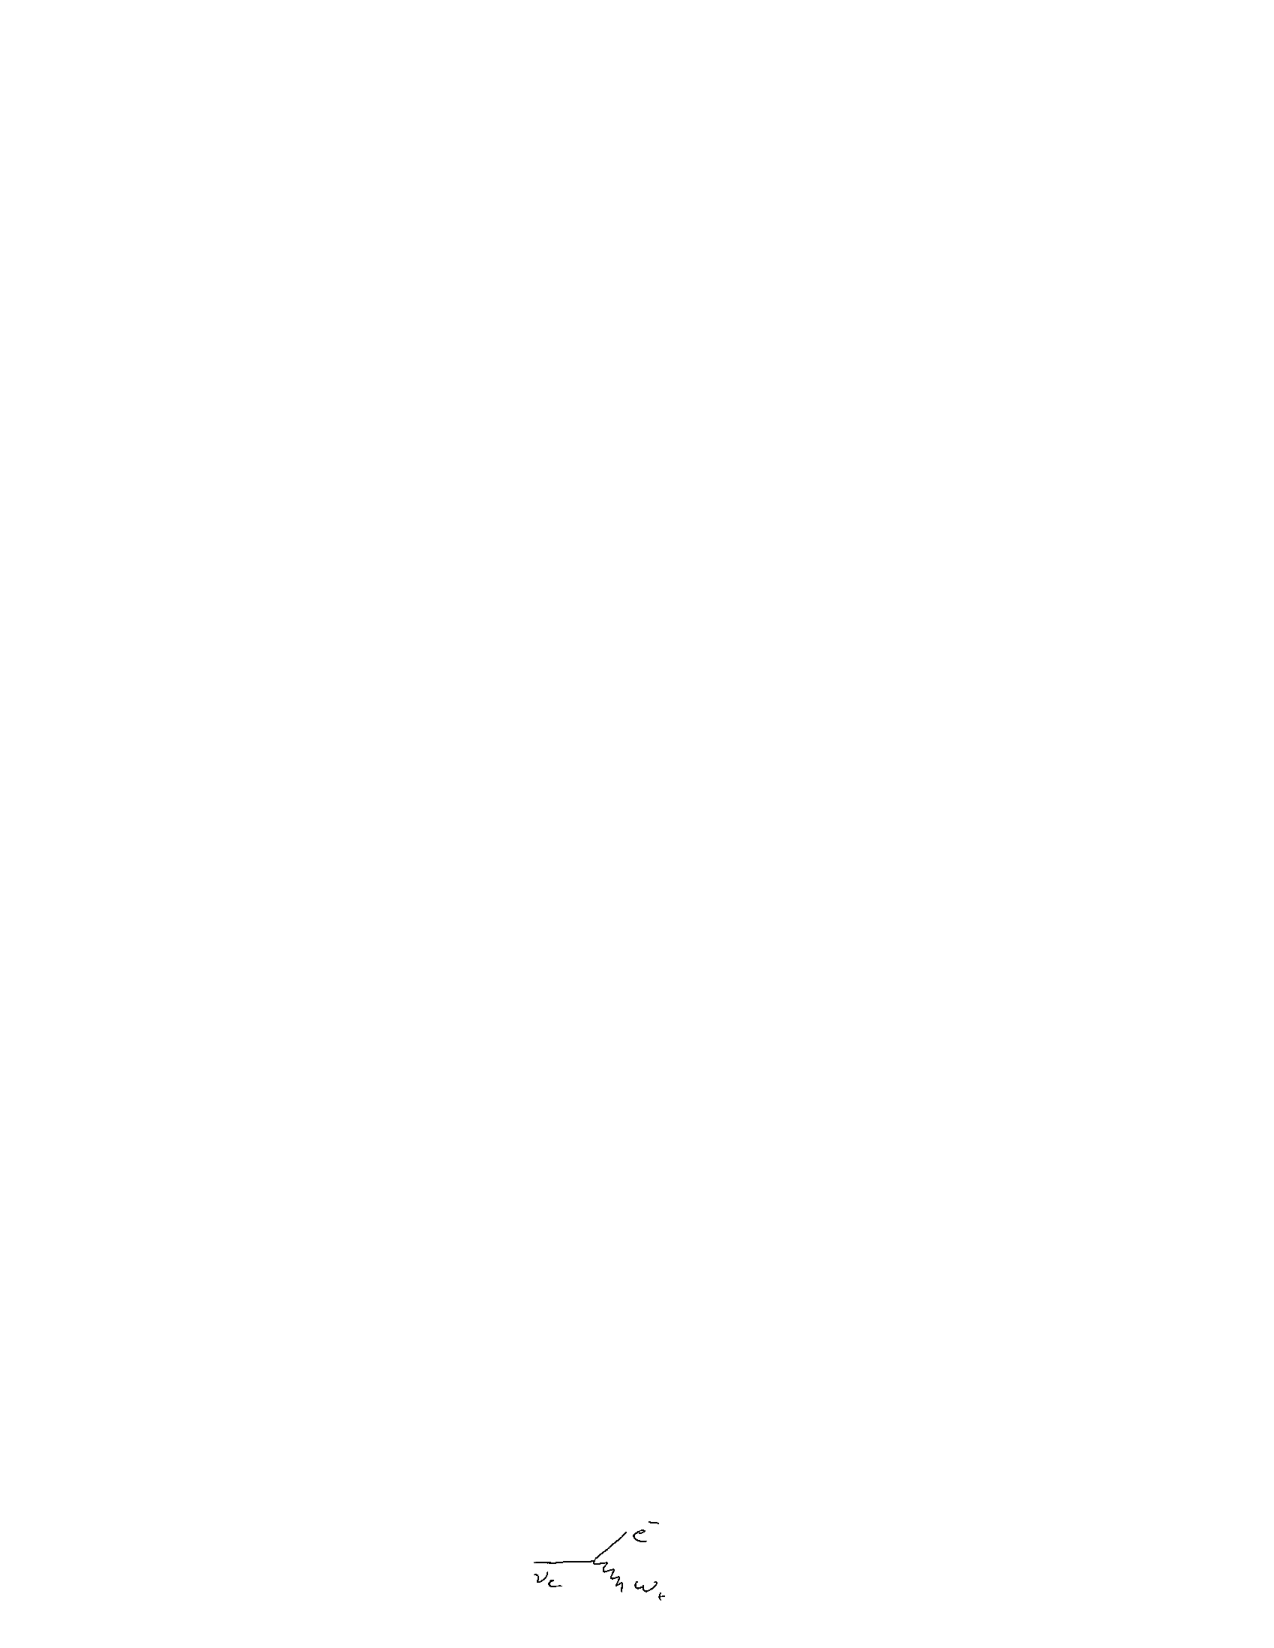
\includegraphics[width=0.2\textwidth]{./wplus.pdf}} + \underbrace{i^2 g e \gamma_\mu W^\mu_- \nu_e }_{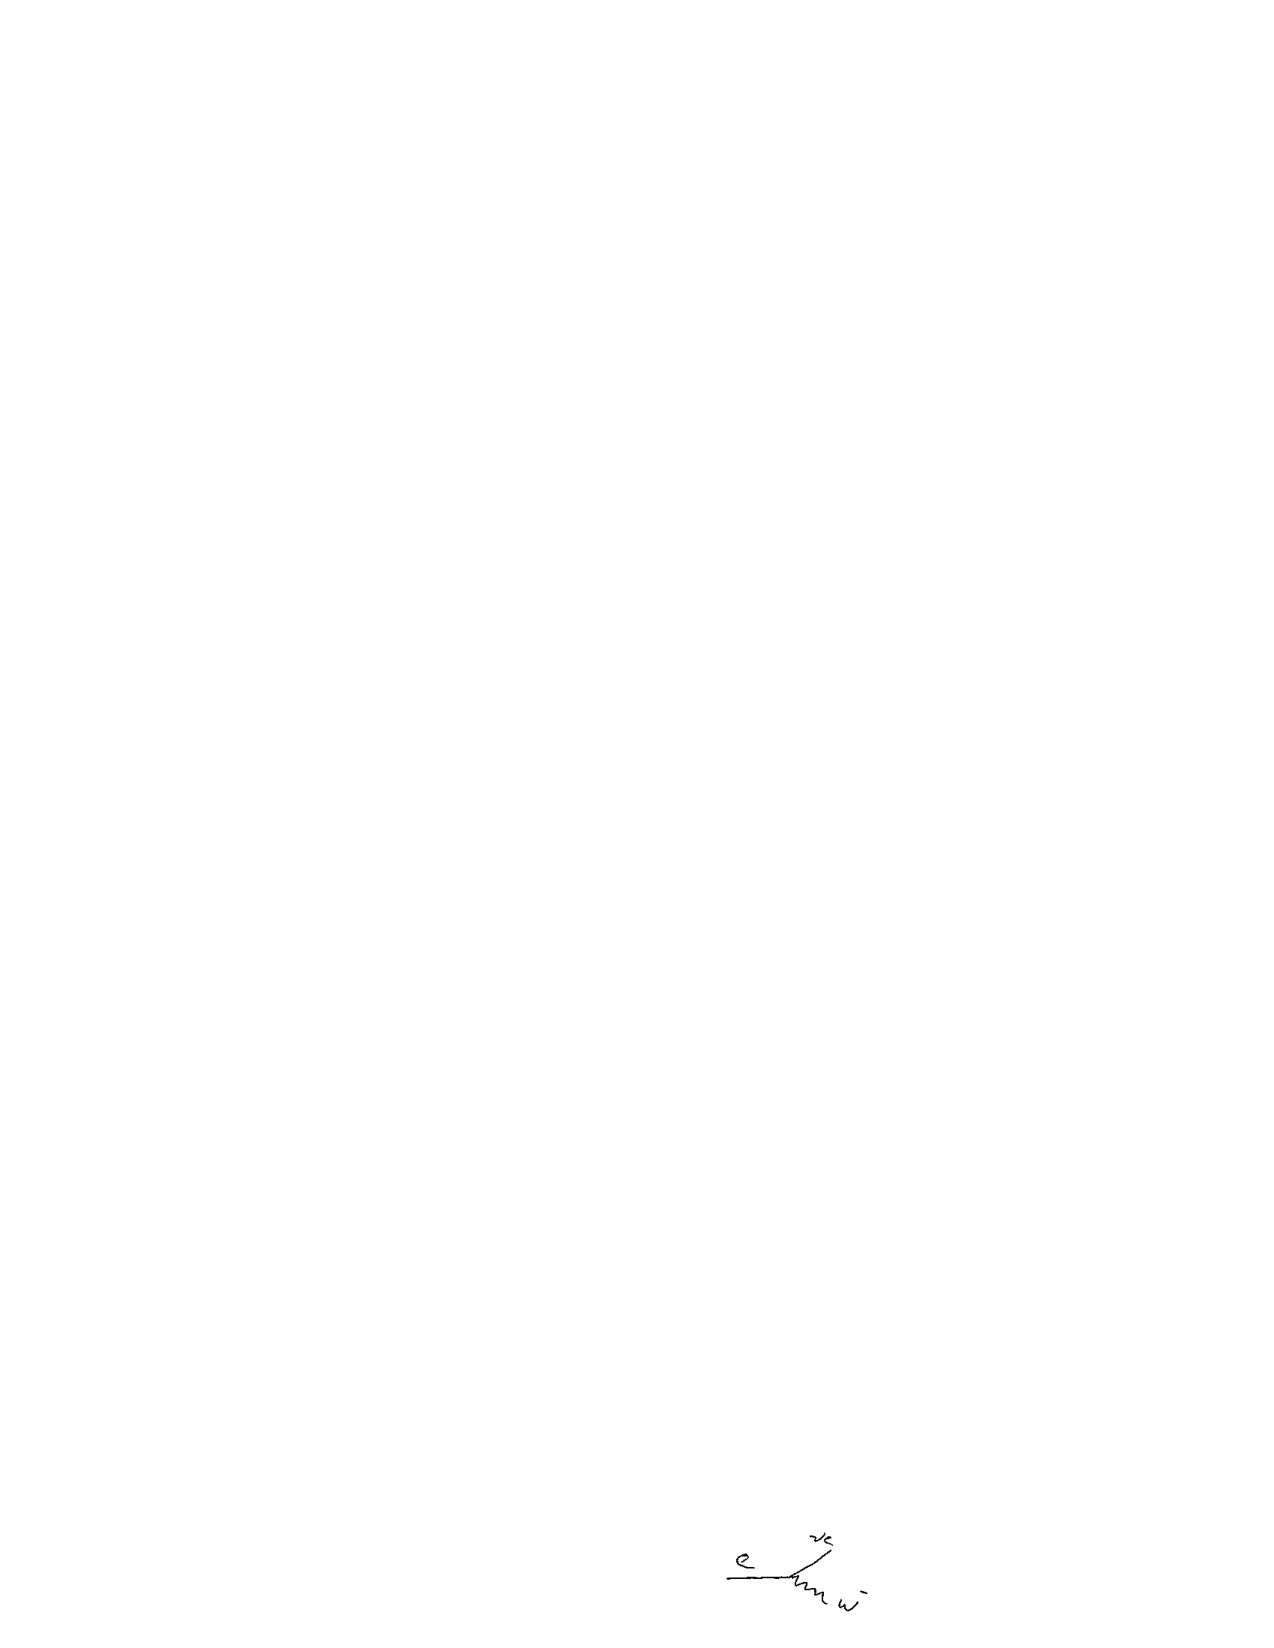
\includegraphics[width=0.2\textwidth]{./wminus.pdf}} \\ 
  &+& \underbrace{i^2 g\nu_e \gamma_\mu W^\mu_3 \nu_e }_{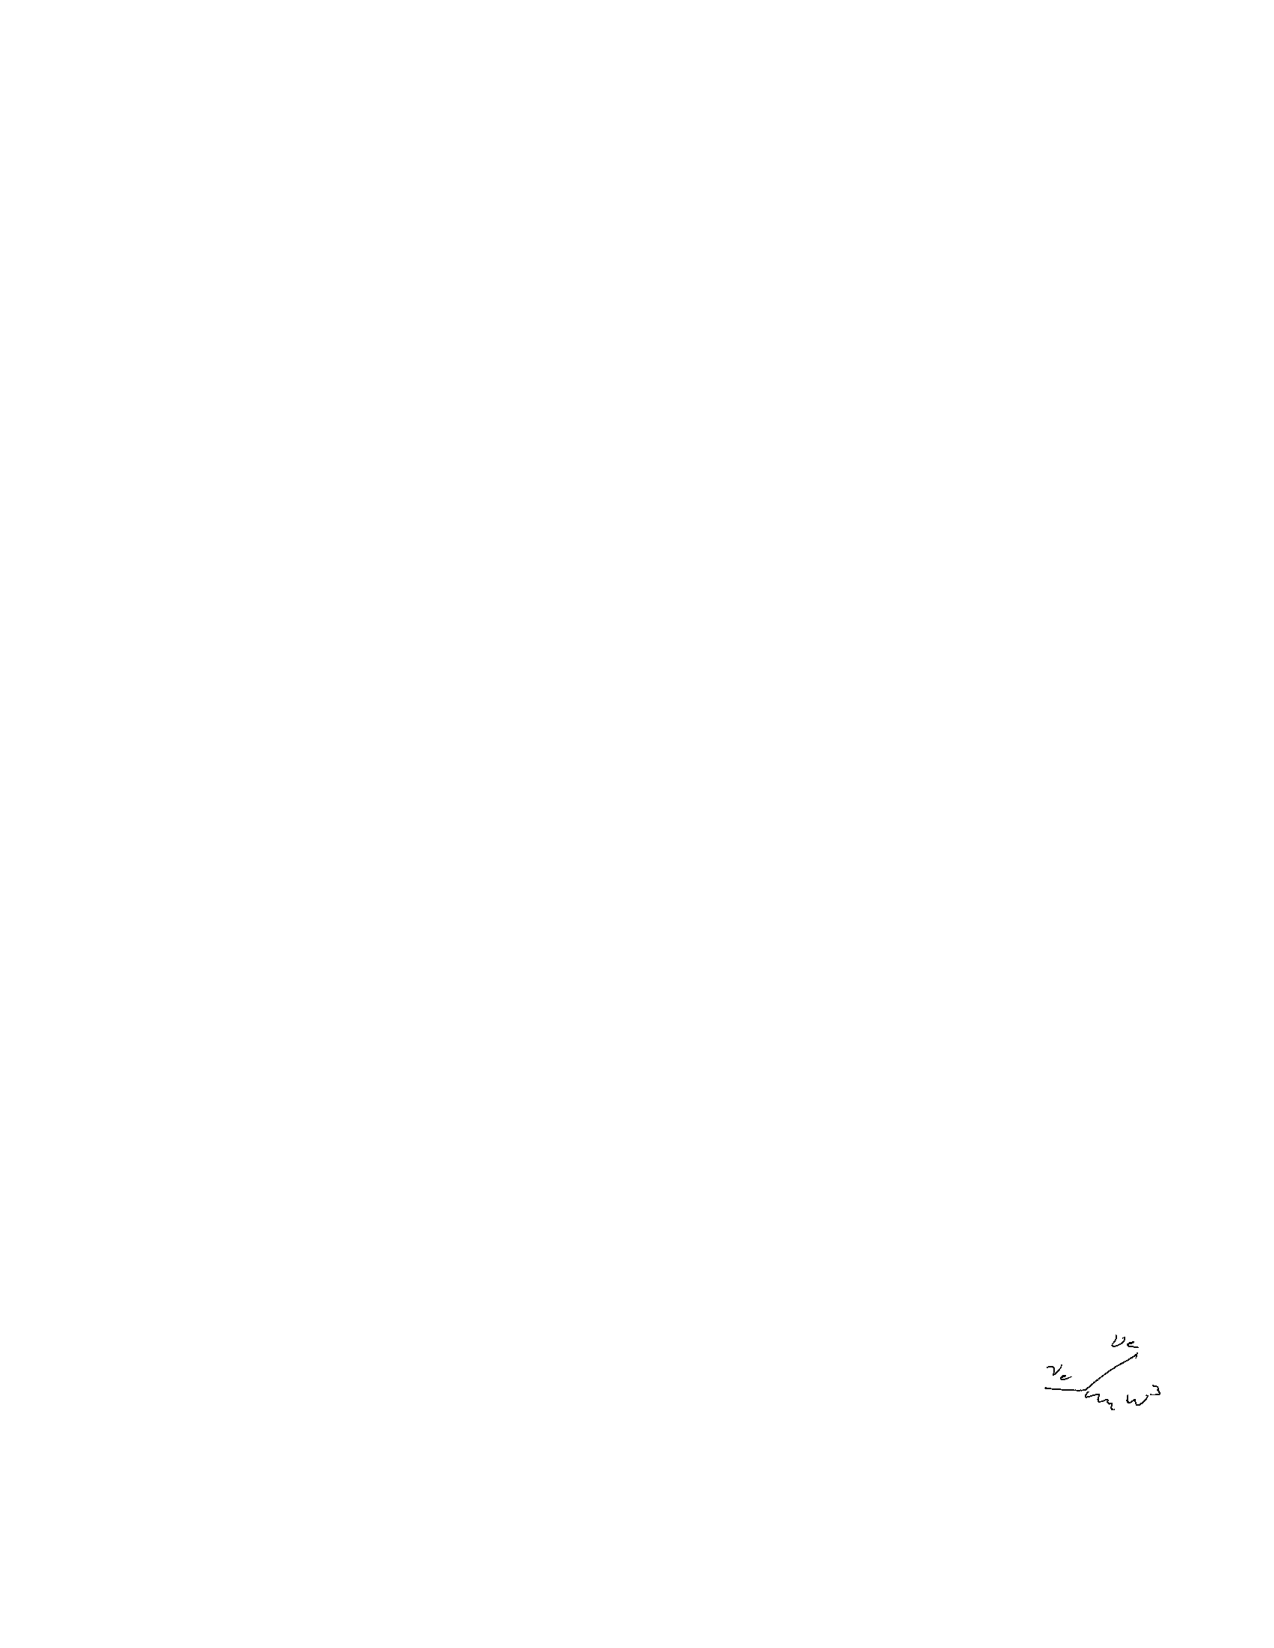
\includegraphics[width=0.2\textwidth]{./w3nu3.pdf}} + \underbrace{i^2 g e \gamma_\mu W^\mu_3 e }_{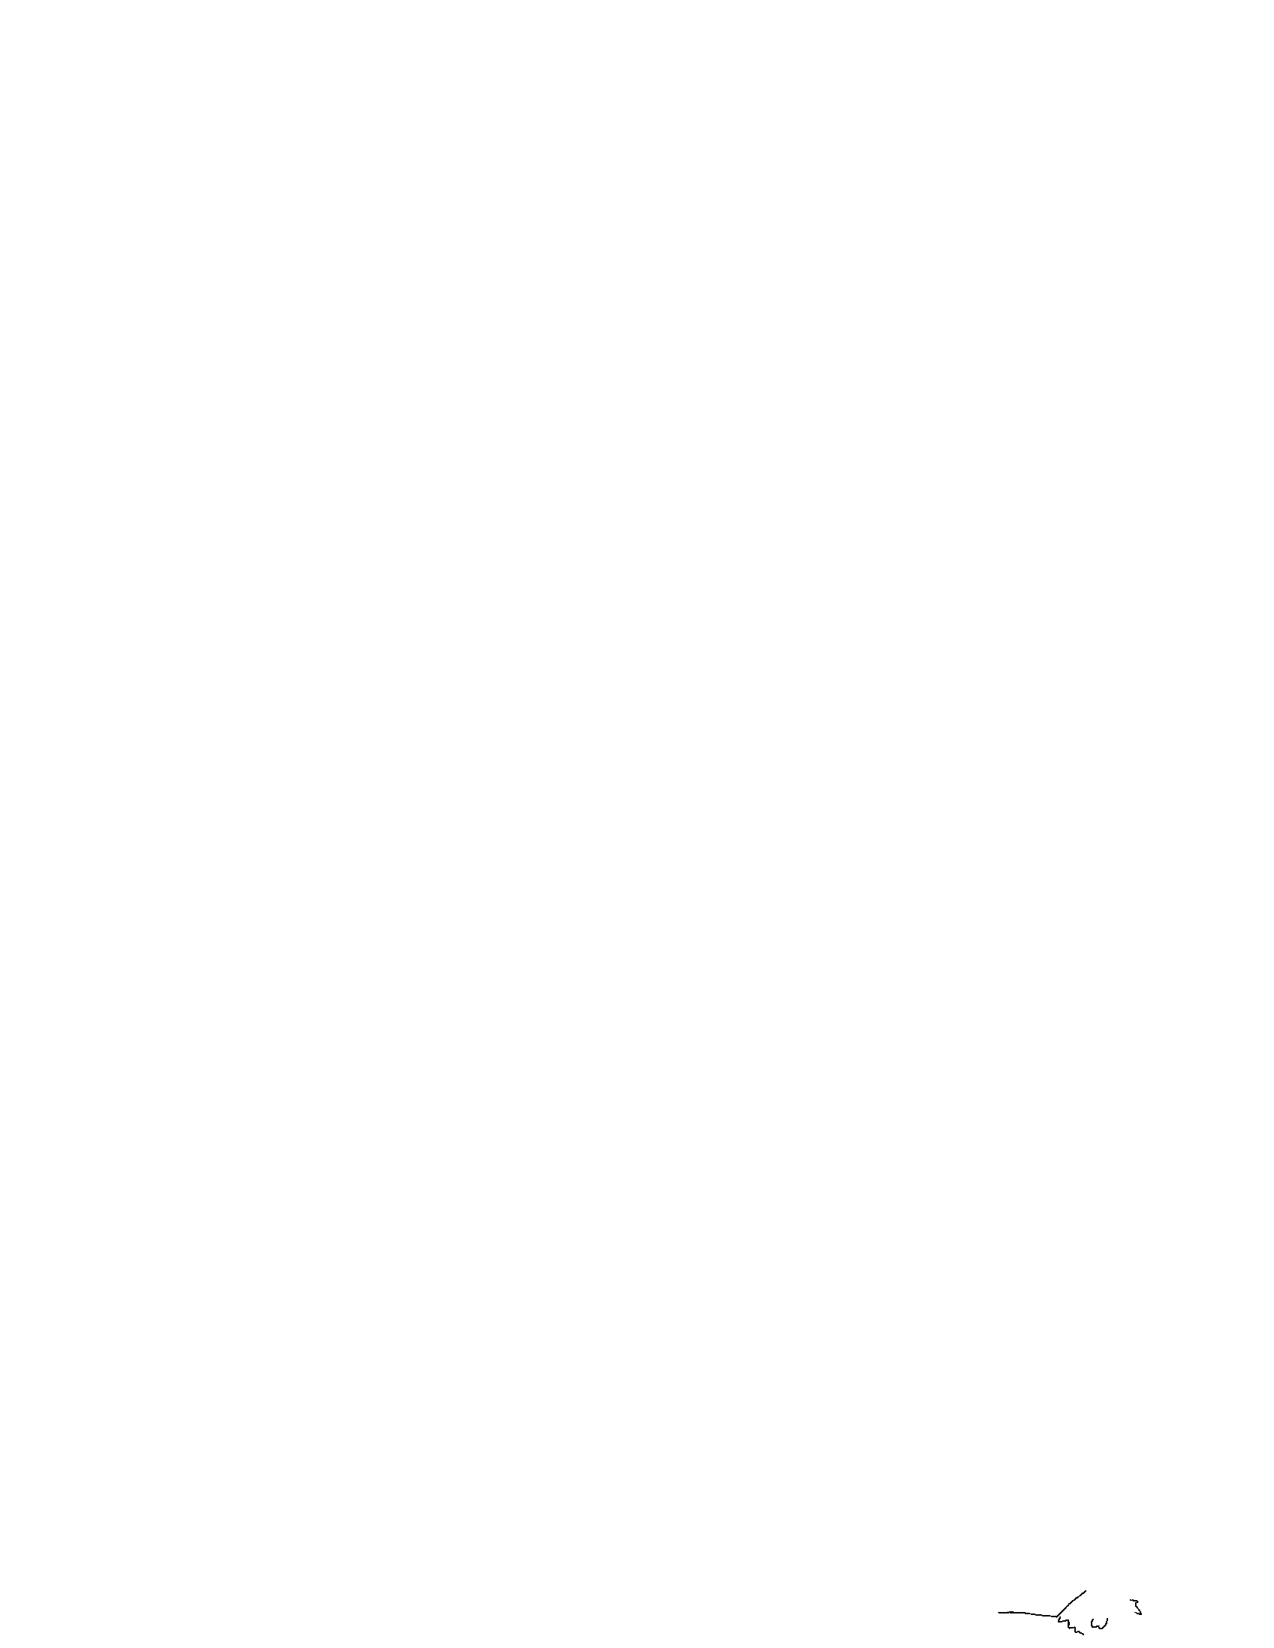
\includegraphics[width=0.2\textwidth]{./w3ee.pdf}}
\eea


\lineacross

\clearpage

Problem is that the weak interaction only talk to left-handed particles. \\
The gauge group is really $SU(2)_L$.

To deal with this only introduce the left handed particles in isospin doublets.

\be
\begin{pmatrix} \nu_e \\ e \end{pmatrix}_L  \hspace*{0.2in}  \begin{pmatrix} \nu_\mu \\ \mu \end{pmatrix}_L \hspace*{0.2in}  \begin{pmatrix} \nu_\tau \\ \tau \end{pmatrix}_L \hspace*{0.2in} \begin{pmatrix} u \\ d \end{pmatrix}_L \hspace*{0.2in}  \begin{pmatrix} c \\ s \end{pmatrix}_L  \hspace*{0.2in} \begin{pmatrix} t \\ b \end{pmatrix}_L
\ee

Treat the Right-handed particles as ``singlets''

\be
e_R \hspace*{0.2in} \mu_R \hspace*{0.2in} \tau_R \hspace*{0.2in} u_R \hspace*{0.2in} d_R \hspace*{0.2in} c_R \hspace*{0.2in} s_R \hspace*{0.2in} t_R \hspace*{0.2in} b_R
\ee 

Under a $SU(2)_L$ gauge transformation 

\be
\phi_R \rightarrow \phi_R  \hspace*{1in}  \phi_L \rightarrow e^{ig\alpha \cdot \sigma} \phi_L
\ee

\textbf{\underline{Weird but true!}} 

\lineacross

Now some history...

Tempting to identify $W^\pm$ with the $W^\pm$ bosons and $W^3$ with the Z boson.

Turns out that that doesn't work. The $W^3$ only couples to left-handed particles, whereas the Z couples to both (although not equally).

However at the time all of this was being sorted out no one had seen $W^\pm$ or Z particles, they only  had the $\gamma$ and the four-point Fermi theory. 

It was believed that this theory needed to be extended to include charged force carriers. 
Mainly through the observation of weak ``charged currents''  $\nu \rightarrow e^2$ or $n \rightarrow p$.

There was no indication of a weak ``neutral current'' $\nu \rightarrow \nu$ (hard to see) or $e \rightarrow e$ (EM dominates).

So the first response to the $SU(2)_L$ theory was that it was just wrong: $W^3$ did not look like the $\gamma$ which couples to both left and right-handed particles. 
Then Glashow-Salam-Weinberg added another group...

\textbf{Add $U(1)_Y$ as new gauge symmetry}

The charge under this group refereed to as ``Hyper-charge''.

So now have $SU(2)_L \times U(1)$ . 

So now, under the full group,
\be
\phi_L \rightarrow e^{ig\alpha \cdot \sigma + i g' y} \phi_L \hspace*{1in} \phi_R \rightarrow e^{ig'y} \phi_R 
\ee
and
\be
\partial_\mu \rightarrow D_\mu = \partial_\mu + ig\vec{W}_\mu \cdot \vec{\sigma} + ig' \underbrace{B_\mu}_{\rmt{New gauge field}}
\ee

Now it looks like we may have enough freedom except, $mee \sim m e_L e_R$ is no longer gauge invariant. 

Because: $e_L \rightarrow e^{ig\vec{\alpha}\sigma}e_L$ under $SU(2)_L$ and $e_R$ doesn't.

So lets just ignore fermion masses for now and just try to give the Bosons masses with the Higgs. 

\lineacross 

Saw two lectures ago how to use the Higgs mechanism to generate mass for a photon in U(1) symmetry. 

Now we will do the same for $SU(2)_L \times U(1)$ ``GSW'' 

\underline{Note} In the Higgs mechanism we are just making things up. 
So there is freedom in what you can do. 
eg: we are just adding fields to $\mathcal{L}$. 
We will go through the simplest case, but again we are putting this in by hand, so it could certainly be something more complicated...


Introduce:
\be
\Phi = \begin{pmatrix} \phi^+ \\ \phi ^0\end{pmatrix}  = \frac{1}{\sqrt{2}} \begin{pmatrix}  \phi_1f + i \phi_2 \\  \phi_3 + i \phi_4 \end{pmatrix}
\ee

\be
\mathcal{L} = (\partial \Phi)^2 - V(\Phi)
\ee
where
\be
V(\Phi) = \mu^2 \Phi^\dagger \Phi + \lambda (\Phi^\dagger \Phi)^2
\ee

$\mu^2 < 0$ has infinite set of degenerate minima satisfying:
\be
\Phi^\dagger \Phi = \frac{1}{2}(\phi_1^2 + \phi_2^2 + \phi_3^2 + \phi_4^2) = \frac{v^2}{2} = \frac{-\mu^2}{2\lambda}
\ee
expand about one of these minima just as we did before. Will pick the ``$\phi_3$ direction''
\be
\phi  \frac{1}{\sqrt{2}} \begin{pmatrix} \phi_1(x) + i \phi_2(x) \\ v + \eta(x) + i\phi_4(x) \end{pmatrix} \underbrace{\rightarrow}_{\rmt{Pick gauge to be}} \phi = \begin{pmatrix} 0 \\ v + h(x) \end{pmatrix}
\ee

Lets see what happens...

Imposing gauge invariance: $\phi \rightarrow e^{ig\vec{\alpha}\sigma}\phi$  and $\partial \rightarrow D$


Need $(D_\mu \Phi)^\dagger (D^\mu \Phi)$ (I will be dropping many factors of 2...)

\be
D_\mu \Phi = (\partial_\mu + ig_W \sigma \cdot W_\mu  + i g' B_\mu) \Phi
\ee

or

\be
\begin{pmatrix} \partial_\mu + ig_w W^3_\mu + ig'B_\mu  & ig_W(W^1_\mu - iW^2_\mu) \\ ig_W(W^1_\mu + iW^2_\mu) & \partial_\mu - ig_w W^3_\mu + ig'B_\mu \end{pmatrix} \begin{pmatrix} 0 \\ v + h \end{pmatrix}
\ee

\be
= \begin{pmatrix} ig_W(W^1_\mu - iW^2_\mu)(v+h) \\ \partial_\mu - ig_w W^3_\mu + ig'B_\mu(v+h) \end{pmatrix}
\ee
from this we can get $(D_\mu\Phi)^\dagger$


\bea
(D_\mu \Phi)^\dagger (D^\mu \Phi) &=& (\partial h)^2 + g_W(W^1_\mu + i W^2_\mu)(W^{1\mu} - i W^{2\mu})(v+h)^2 \\
 &+& (g_wW^3_\mu - g'B_\mu)(g_WW^{3\mu} - g'B^\mu)(v+h)^2
\eea


Lets look at the terms that go like $v^2$

\be
g_W^2 v^2 (W^1_\mu + i W^2_\mu)(W^{1\mu} - i W^{2\mu}) = \underbrace{v^2 g_W^2 }_{m_W^2} ({W^1}^2 + {W^2}^2)
\ee

$\Rightarrow$ $W^1$ and $W^2$ are massive with mass $m_W = g_Wv$ (Same mass!)

There is also a term like
\be
v^2 (g_wW^3_\mu - g'B_\mu)(g_WW^{3\mu} - g'B^\mu) 
\ee
which can be written as

\be
= v^2 \begin{pmatrix} W_\mu^3 & B_\mu \end{pmatrix} \underbrace{\begin{pmatrix} g_W^2 & -g_W g' \\ -g_Wg' & g'^2 \end{pmatrix}}_{\rmt{M - non-diagonal mass matrix} }    \begin{pmatrix} W_\mu^3 \\ B_\mu \end{pmatrix}
\ee

This non-diagonal mass matrix is telling you that the $W_\mu^3$ and $B_\mu$ fields ``mix''.


So pure $W_\mu^3$ or $B_\mu$ has probability to turn into the other. 
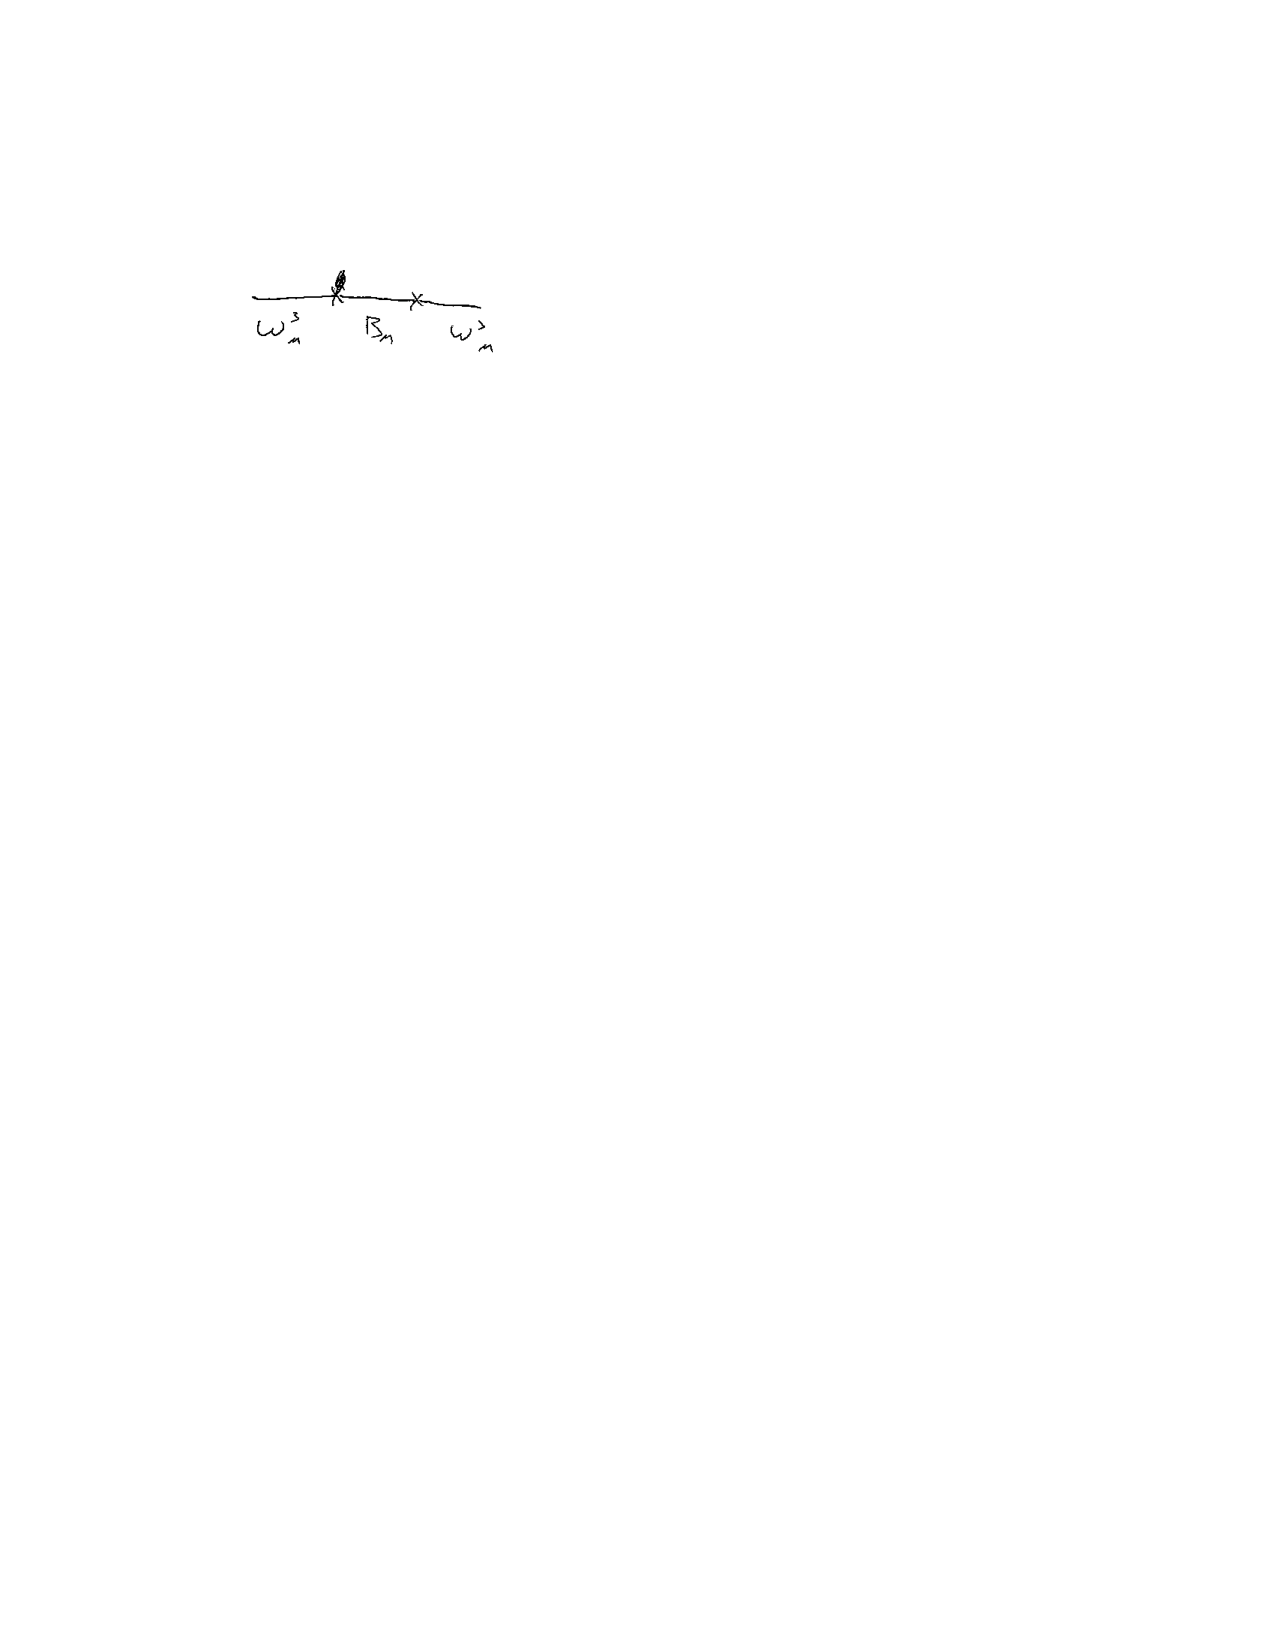
\includegraphics[width=0.2\textwidth]{./WandBMixing.pdf}

These are not eigenstates of the free Hamiltonian.

Need to solve for the linear combination of $W^3$ and $B$ which diagonalizes M.

These linear combinations would \multiline{1) not mix \\ 2) Have definite mass \\ 3) Be energy eigenstates} 


Solve $det(M-\lambda I ) = 0$

\be
\Rightarrow (g_W^2 - \lambda)(g'^2 - \lambda) - g_W^2 g'^2 = 0
\ee
Gives, $\lambda = 0$ or $\lambda = g_W^2 + g'^2$

In diagonal basis,

\be
v^2 \begin{pmatrix} A_\mu & Z_\mu \end{pmatrix}  \begin{pmatrix} 0 & 0 \\ 0 & g_W^2 + g'^2 \end{pmatrix}  \begin{pmatrix} A_\mu \\ Z_\mu \end{pmatrix}  
\ee

Where $A_\mu$ and $Z_\mu$ are the eigenvectors

\be
\underbrace{A_\mu = \frac{1}{\sqrt{g_W^2 + g'^2}}(g'W_\mu^3 + g_W B_\mu)}_{\rmt{\huge $m_A = 0$}} \hspace*{0.5in} \underbrace{Z_\mu = \frac{1}{\sqrt{g_W^2 + g'^2}}(g_W W_\mu^3 - g' B_\mu)}_{\rmt{\huge $m_Z = v^2\sqrt{g_W^2 + g'^2}$}}
\ee

There is also a term that goes like $h^2$ (Homework)

\lineacross

Recap:  

Start with:  
\be
\underbrace{\phi_1, \hspace*{0.2in} \phi_2, \hspace*{0.2in} \phi_3, \hspace*{0.2in} \phi_4}_{\rmt{DoF: $4\times 1$ (scalars) }}, \hspace*{0.2in} \underbrace{W^1, \hspace*{0.2in} W^2, \hspace*{0.2in}W^3, \hspace*{0.2in} B}_{\rmt{$4\times 2$ (mass-less spin-1)}}
\ee                 
So 12 total degrees of freedom.

When $\mu^2 < 0$, left with


\be
\underbrace{h}_{\rmt{DoF: 1}} \hspace*{0.3in} \underbrace{W^+ \hspace*{0.3in} W^- \hspace*{0.3in} Z}_{\rmt{$3 \times 3$ (massive spin 1) }} \hspace*{0.3in} \underbrace{\gamma}_{2}
\ee

Total degrees of freedom 12, as needed!


}
\end{document}


